\section{Ziele}
\label{sec:ziele}
Es soll zuerst die Bragg Bedingung an einem LiF Kristall überprüft werde.
Außerdem soll im Experiment das Kupfer Röntgenspektrum gemessen, dargestellt und analysiert werden.
Im letzten teil des Versuchs soll die Absorption von verschiedenen Metallen untersucht werden.
\section{Theoretische Grundlagen}
\label{sec:theorie}

\subsection{Erzeugung von Röntgenstrahlung}
\subsubsection{Bremsspektrum}
\begin{figure}
    \centering
    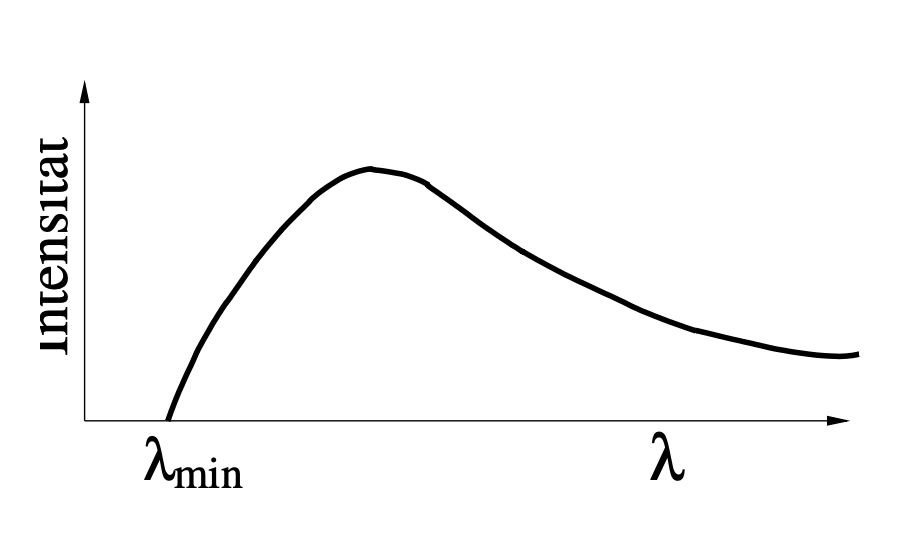
\includegraphics[width=0.7\textwidth]{bilder/Bremsspektrum.png}
    \caption{Skizze eines Graphen der die Intensität der Röntgenstrahlung in abhängigkeit von der Wellenlänge zeigt. (Quelle \cite{Anleitung})}
    \label{fig:Bremsspektrum}
\end{figure}
\subsubsection{Charakteristische Peaks}

\subsection{Absorption}
\begin{figure}
    \centering
    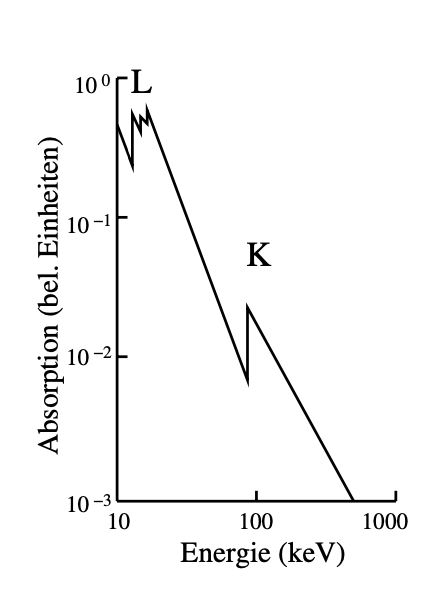
\includegraphics[width=0.7\textwidth]{bilder/Absorption.png}
    \caption{Skizze eines Graphen für das auftragen der Absorption gegen die Energie. Auf der Skizze sind die gut erkenntlichen L und K Kanten beschriftet. (Quelle \cite{Anleitung})}
    \label{fig:Absorption}
\end{figure}

\subsection{Bragg Reflexion}
\begin{figure}
    \centering
    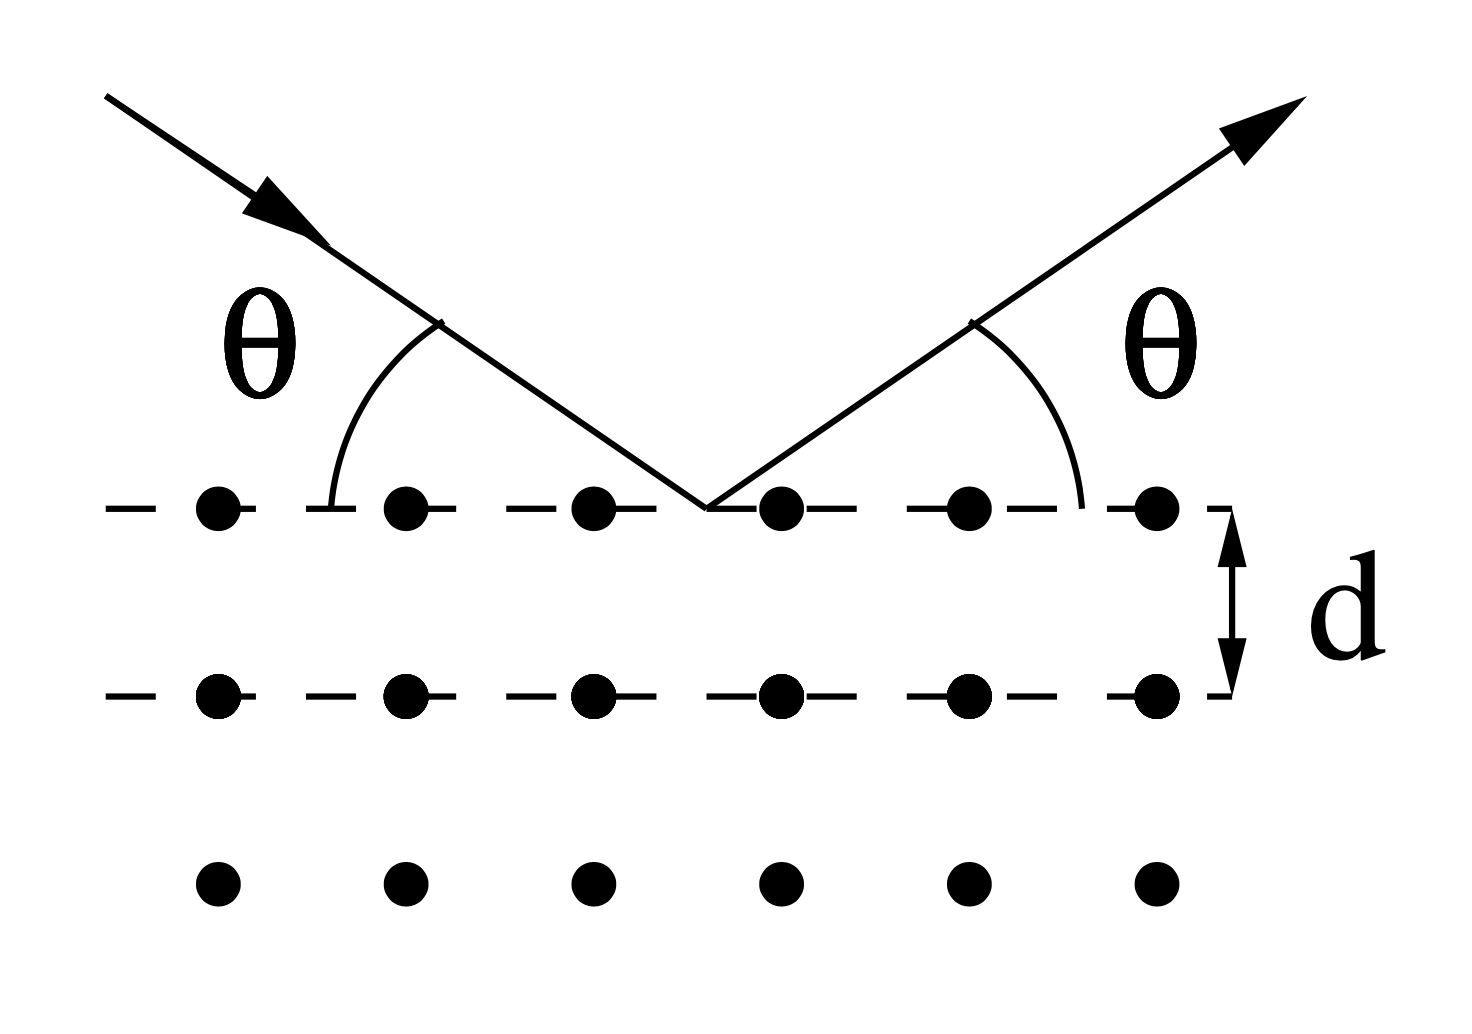
\includegraphics[width=0.7\textwidth]{bilder/Bragg_Reflexion.png}
    \caption{Eine schematische Skizze der Bragg Reflexion. (Quelle \cite{Anleitung}}
    \label{fig:Bragg_Reflexion}
\end{figure}
